\section{Database}\label{sec:database}
Il modello descrive il DDL PostgreSQL corrente di \code{schema.sql},
riscontrato con mapping DAO e dominio: comprende tredici tabelle,
quindici chiavi esterne, una vista delle identità e una sequenza comune
agli utenti applicativi. Non è derivato dalle classi Java né ottenuto
da un'esportazione automatica. Le tavole distinguono il modello delle
relazioni dai controlli che richiedono la collaborazione dei servizi.

\subsection{Schema ER}
La figura~\ref{fig:er-autori} riprende \emph{SWE ER}, la tavola degli
autori, conservando tabelle a tre colonne, disposizione, generalizzazione
e cardinalit\`a a zampa di corvo. Sono aggiornati campi, tipi enumerati e
unicit\`a della richiesta per veicolo. Il nodo \emph{User} resta un
supertipo \textbf{concettuale}: non rappresenta una tabella padre, una PK
globale o un vincolo SQL di disgiunzione. Gli attributi comuni sono
ripetuti nelle tre tabelle di ruolo; PK e unicit\`a dell'email sono locali
a ciascuna. La seconda pagina conserva e corregge legenda e note.
Le due pagine A3 mantengono leggibile la tavola d'insieme; ER-01/02 e
REL-01--03 dettagliano poi relazioni, mapping e limiti dello schema.
\tavolaautori{database-er-autori}{Schema ER: tavola degli autori corretta, con notazione e gerarchia concettuale originali}{fig:er-autori}

Le viste ER-01 e ER-02 (figure~\ref{fig:er01} e~\ref{fig:er02}) sono
coordinate: i riquadri ripresi con lo stesso nome indicano la stessa
entità. Ogni arco dichiara entrambi i versi con minimo e massimo,
ricavati da nullabilità, unicità e FK, senza dedurli da riferimenti Java.
La parte catalogo collega marca, modello, veicolo e sconti. Ogni modello
ha una marca e ogni veicolo un modello; il padre può non avere figli.
Uno sconto appartiene a un solo modello o veicolo; la chiave condivisa
consente al padre zero o uno sconto.

Una richiesta riguarda esattamente un cliente e un veicolo; l'unicità
di \code{request.vehicle} limita a una la richiesta aperta per veicolo,
indipendentemente dal tipo. Il venditore è facoltativo. Test drive e
noleggio hanno entrambi cliente e veicolo obbligatori, con più operazioni
possibili nel tempo. Nel registro economico il cliente rimane obbligatorio,
mentre veicolo e venditore sono opzionali: il primo può anche essere
azzerato dalla cancellazione del veicolo. La penale prodotta dal servizio
non riferisce né veicolo né venditore; lo schema non impone questa
combinazione in funzione del tipo.

La vista ER delle identità mantiene le tre tabelle effettive, senza
inventare una tabella padre \code{user}. Il manager non è bersaglio di
FK applicative. Ogni conto appartiene a un cliente; \code{UNIQUE(client)}
consente a ciascun cliente al massimo un conto, ma nessuna FK impone
che ogni cliente ne possieda uno. La creazione congiunta è una scelta
transazionale di \code{AuthService}, non una partecipazione minima SQL.

\begin{figure}[p]
  \centering
  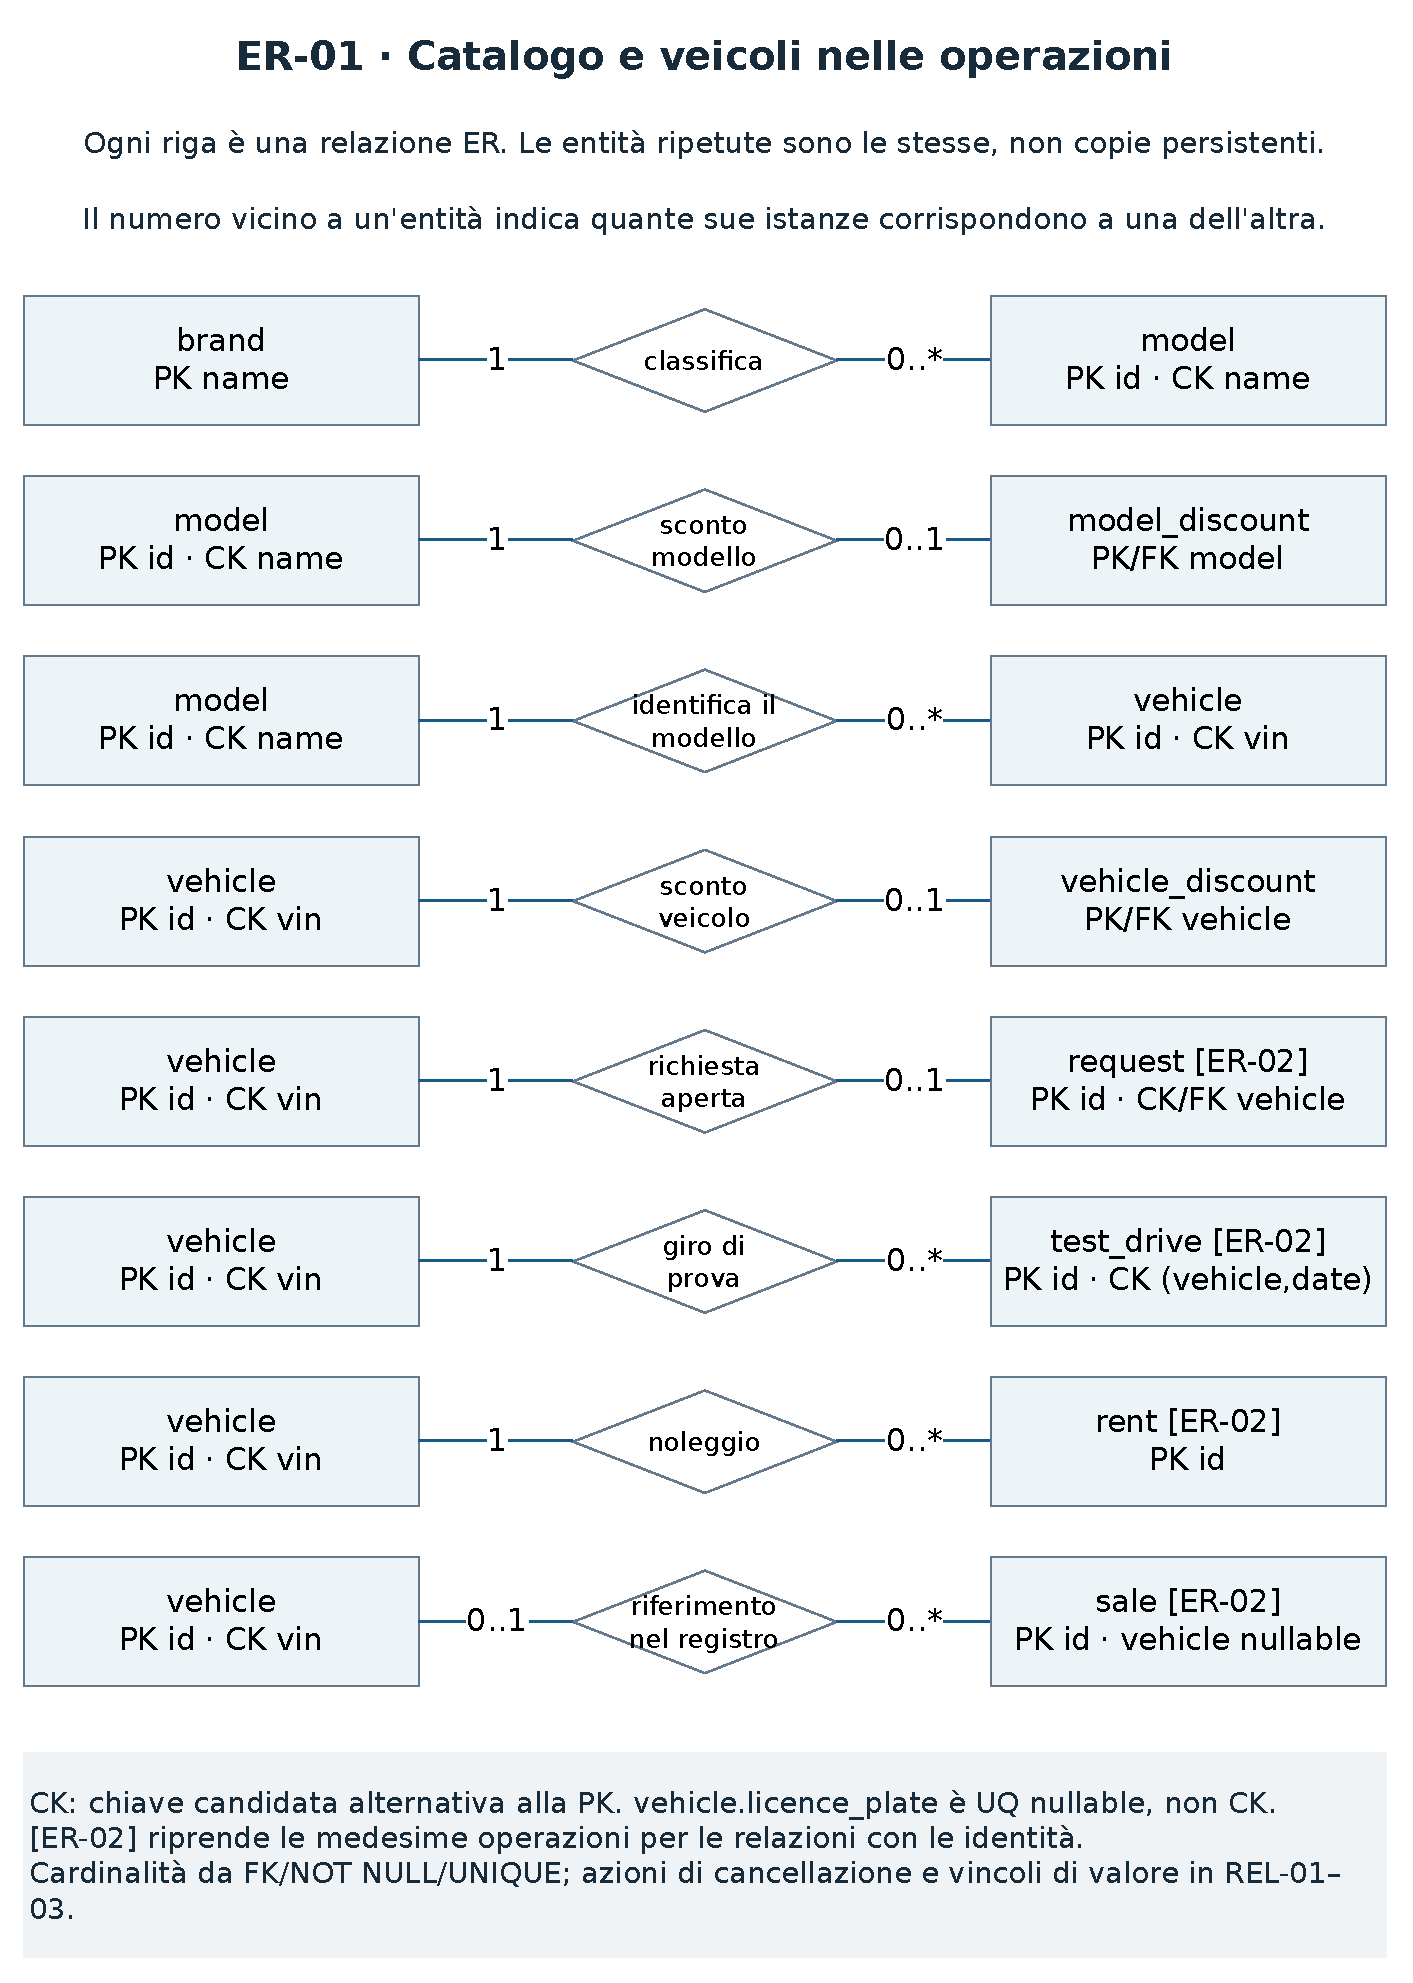
\includegraphics[width=\linewidth,height=.88\textheight,keepaspectratio]{diagrammi/database-er-catalogo.drawio.pdf}
  \caption{ER-01 --- Catalogo e riferimenti dei veicoli nelle operazioni; cardinalità nei due versi.}\label{fig:er01}
\end{figure}
\begin{figure}[p]
  \centering
  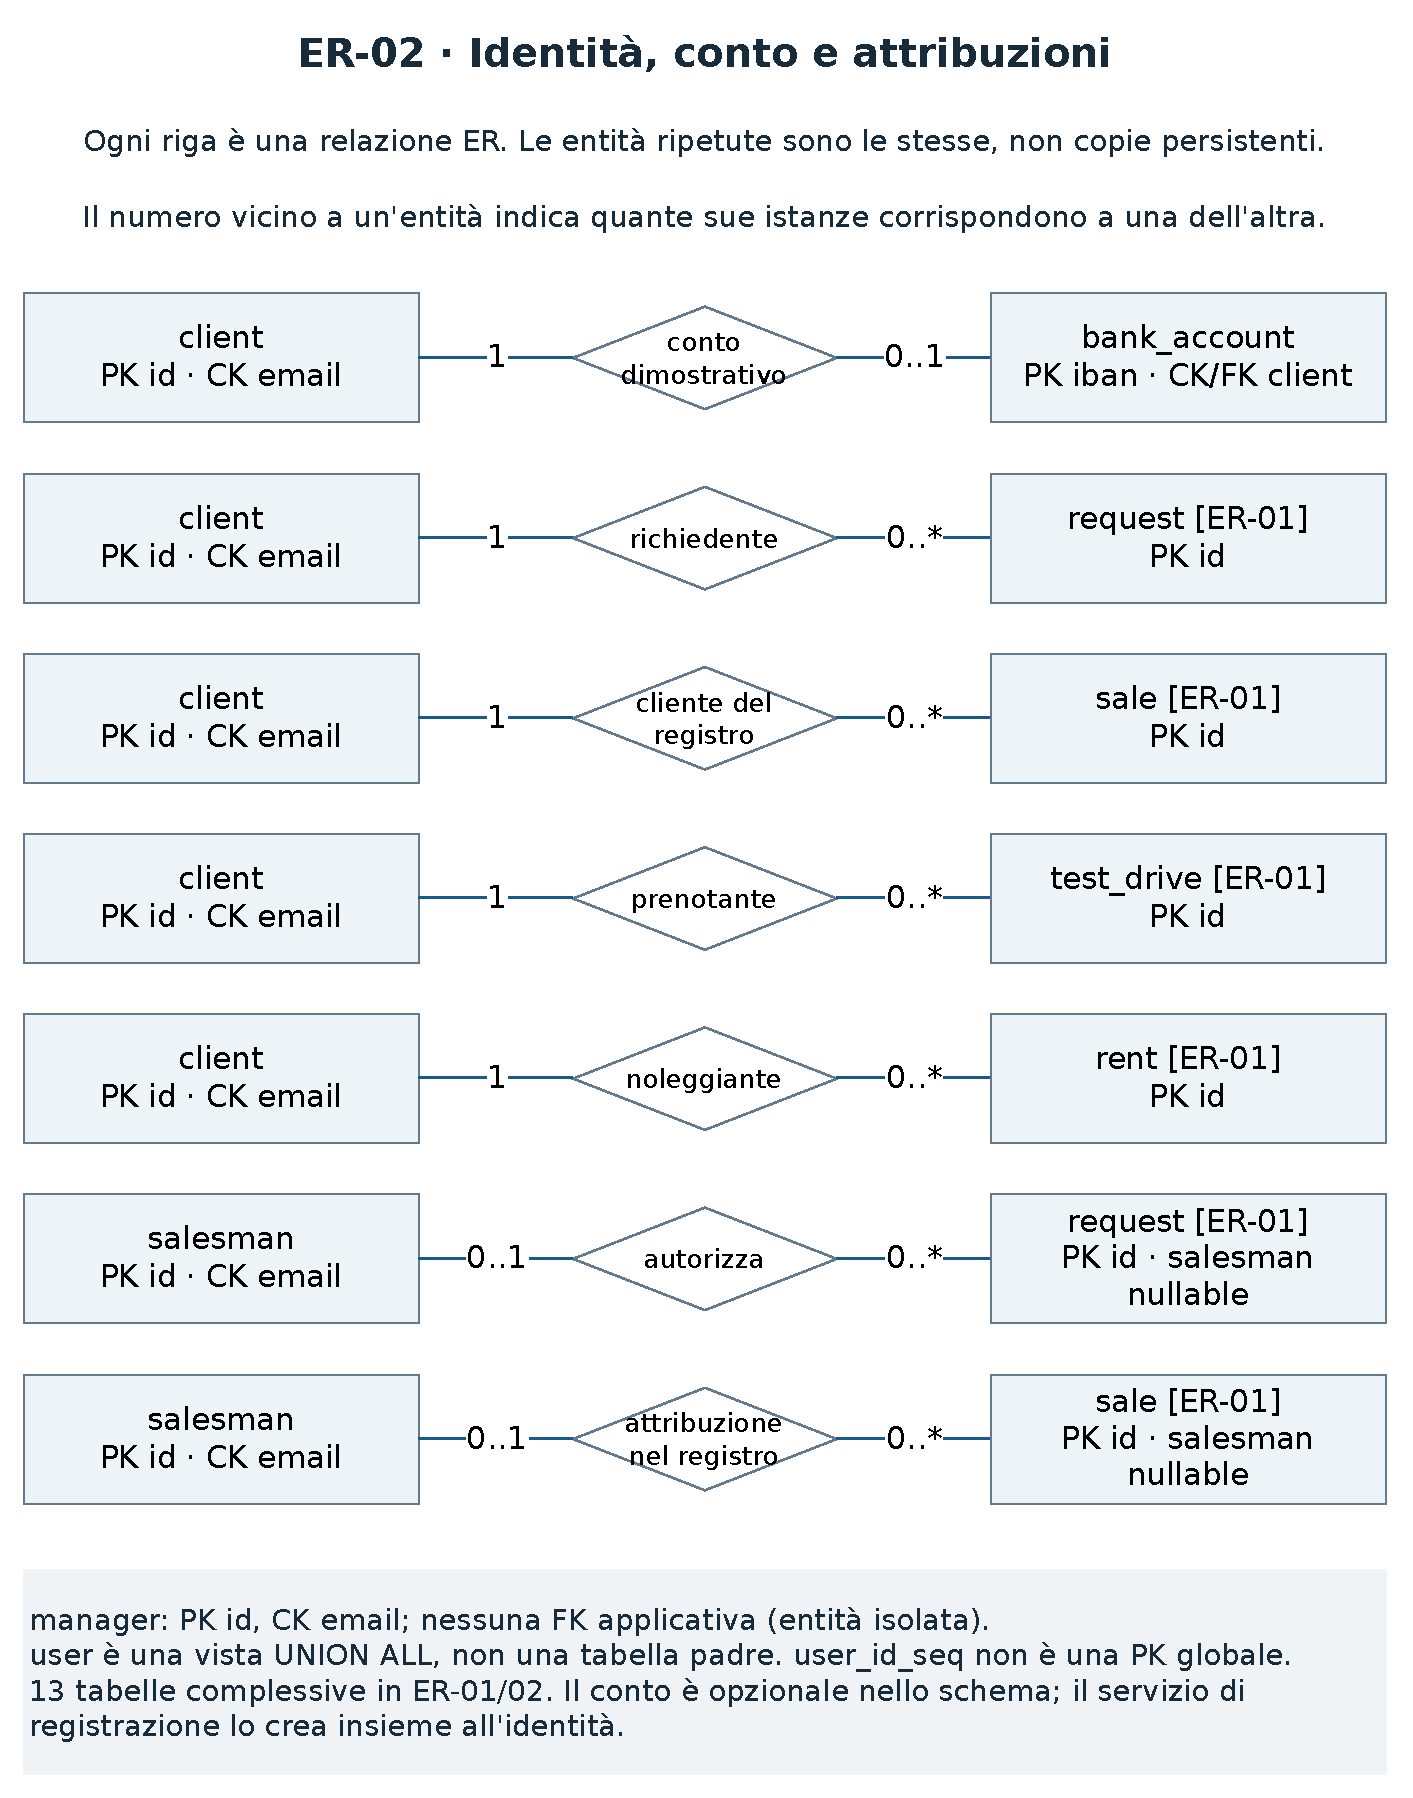
\includegraphics[width=\linewidth,height=.88\textheight,keepaspectratio]{diagrammi/database-er-identita.drawio.pdf}
  \caption{ER-02 --- Identità, conto e attribuzioni; le operazioni riprendono ER-01.}\label{fig:er02}
\end{figure}
\clearpage

\subsection{Modello relazionale}
REL-01--REL-03 (figure~\ref{fig:rel01}--\ref{fig:rel03}) riportano
tutti gli attributi, i tipi, le chiavi e i riferimenti. \code{PK} indica
la primaria; \code{CK} una candidata alternativa; \code{FK} un riferimento;
\code{?} la nullabilità. In assenza di \code{?} l'attributo è obbligatorio,
anche quando lo rende tale la primaria. Gli ID di catalogo e operazioni
sono \texttt{BIGINT GENERATED BY DEFAULT AS IDENTITY}; marca e conto
usano rispettivamente nome e IBAN. Gli sconti usano la FK come PK.

\noindent\textbf{Le tredici relazioni, nella notazione testuale.}
\code{PK} indica la primaria, \code{FK} la chiave esterna, \code{U} l'unicità.
Il suffisso \code{?} ammette \code{NULL}; tutti gli altri attributi sono
obbligatori. Una chiave può essere insieme \code{PK} e \code{FK}.
Gli importi sono \code{DECIMAL(10,2)}, gli ID \code{BIGINT}; tipi e lunghezze
completi sono nelle tavole REL. Il simbolo di unicità può riguardare anche
una combinazione di attributi, specificata dopo la relazione.
\begin{description}[style=nextline,leftmargin=1em]
\item[\code{brand}]
(\code{PK name}).
Nome fino a 50 caratteri, chiave usata dai modelli.
\item[\code{model}]
(\code{PK id}, \code{FK brand}, \code{U name}, \code{release_price}, \code{release_year}).
\code{brand} riferisce \code{brand.name}; nome unico globalmente, base non negativa e anno almeno 1900.
\item[\code{model_discount}]
(\code{PK/FK model}, \code{value}).
\code{model} riferisce \code{model.id}; una percentuale intera 0--50 per modello, facoltativa per il padre.
\item[\code{vehicle}]
(\code{PK id}, \code{FK model}, \code{U vin}, \code{U licence_plate?}, \code{kilometers}, \code{price}, \code{price_mode}, \code{year}, \code{state}).
\code{model} riferisce \code{model.id}. VIN fino a 17 caratteri, targa fino a 10; base e chilometri non negativi. \code{price_mode} è predefinito \code{AUTOMATIC}; stato e modalità usano enum distinti. Anno almeno 1900 e non prima del modello; targa assente solo a chilometri zero.
\item[\code{vehicle_discount}]
(\code{PK/FK vehicle}, \code{value}).
\code{vehicle} riferisce \code{vehicle.id}; una percentuale intera 0--50 per veicolo, facoltativa per il padre.
\item[\code{client}]
(\code{PK id}, \code{name}, \code{surname}, \code{U email}, \code{hash_password}).
Nome, cognome ed email fino a 50 caratteri, hash fino a 255. ID predefinito dalla sequenza \code{user_id_seq}; controllo minimo sulla forma dell'email.
\item[\code{salesman}]
(\code{PK id}, \code{name}, \code{surname}, \code{U email}, \code{hash_password}).
Stessi tipi, sequenza e controlli del cliente; primaria e unicità dell'email sono locali alla tabella del venditore.
\item[\code{manager}]
(\code{PK id}, \code{name}, \code{surname}, \code{U email}, \code{hash_password}).
Stessi tipi, sequenza e controlli del cliente; nessuna FK applicativa punta al manager.
\item[\code{bank_account}]
(\code{PK iban}, \code{FK/U client}, \code{balance}).
IBAN fino a 27 caratteri, cliente riferito a \code{client.id}; saldo non negativo, predefinito zero. L'unicità non impone un conto a ogni cliente.
\item[\code{request}]
(\code{PK id}, \code{FK/U vehicle}, \code{FK client}, \code{FK salesman?}, \code{deposit}, \code{agreed_total?}, \code{exp_date?}, \code{type}).
FK a \code{vehicle.id}, \code{client.id}, \code{salesman.id}. Una richiesta aperta per veicolo; scadenza \code{DATE}, tipo \code{request_type}. \code{SALE}: totale obbligatorio non negativo e acconto tra zero e totale; \code{PURCHASE}: stima non negativa e totale nullo.
\item[\code{test_drive}]
(\code{PK id}, \code{FK vehicle}, \code{FK client}, \code{date}).
FK a \code{vehicle.id} e \code{client.id}; data \code{TIMESTAMP}. \code{UNIQUE(vehicle,date)} rende unico il timestamp per veicolo; ora compresa fra 09:00 e 16:00 inclusi.
\item[\code{rent}]
(\code{PK id}, \code{FK vehicle}, \code{FK client}, \code{amount}, \code{start}, \code{end}).
FK a \code{vehicle.id} e \code{client.id}; importo non negativo, estremi \code{DATE} con fine non prima dell'inizio. \code{EXCLUDE} impedisce intersezioni degli intervalli inclusi per lo stesso veicolo.
\item[\code{sale}]
(\code{PK id}, \code{FK vehicle?}, \code{FK salesman?}, \code{FK client}, \code{amount}, \code{date}, \code{type}).
FK a \code{vehicle.id}, \code{salesman.id}, \code{client.id}; importo non negativo, data \code{TIMESTAMP}, tipo \code{sale_type}: \code{SALE}, \code{PURCHASE}, \code{PENALTY}. Nessuna FK alla richiesta consumata.
\end{description}
La vista \code{user(id,name,surname,email,hash_password,role)} combina le
identità con \code{UNION ALL}; il ruolo è una costante di ciascun ramo,
non una quattordicesima tabella. Nullabilità e azioni di cancellazione sono
proprietà distinte: una FK nullable non implica \code{SET NULL}.

Le candidate alternative sono \code{model.name}, \code{vehicle.vin},
le email all'interno di ciascuna tabella di ruolo,
\code{bank\_account.client}, \code{request.vehicle} e la coppia
\code{(vehicle,date)} del test drive: tutte sono uniche e non nulle.
Il nome del modello è unico globalmente, non soltanto entro una marca.
\code{vehicle.licence\_plate} ha invece un vincolo \code{UNIQUE} ed è
nullable: più valori nulli sono ammessi e non è una chiave candidata
dell'intera relazione. Le unicità testuali non implicano da sole
normalizzazione o confronto senza distinzione fra maiuscole e minuscole.

Le azioni \texttt{ON DELETE} sono specifiche. Gli sconti seguono in
\code{CASCADE} il proprio modello o veicolo; il conto segue il cliente.
\code{sale.vehicle} usa \texttt{SET NULL}, conservando la registrazione.
Le altre undici FK usano \code{RESTRICT}: marca con modelli, modello
con veicoli, riferimenti di richieste, test drive e noleggi, cliente e
venditore del registro. Di conseguenza un veicolo con un noleggio o un
test drive non è eliminabile per il solo fatto che \code{sale.vehicle}
consenta \texttt{SET NULL}. L'unico \texttt{ON UPDATE CASCADE} è
\code{model.brand}; le altre FK mantengono il predefinito \texttt{NO ACTION}.
I servizi aggiungono controlli conservativi sullo storico, senza cambiare
queste regole SQL.

\begin{figure}[p]
  \centering
  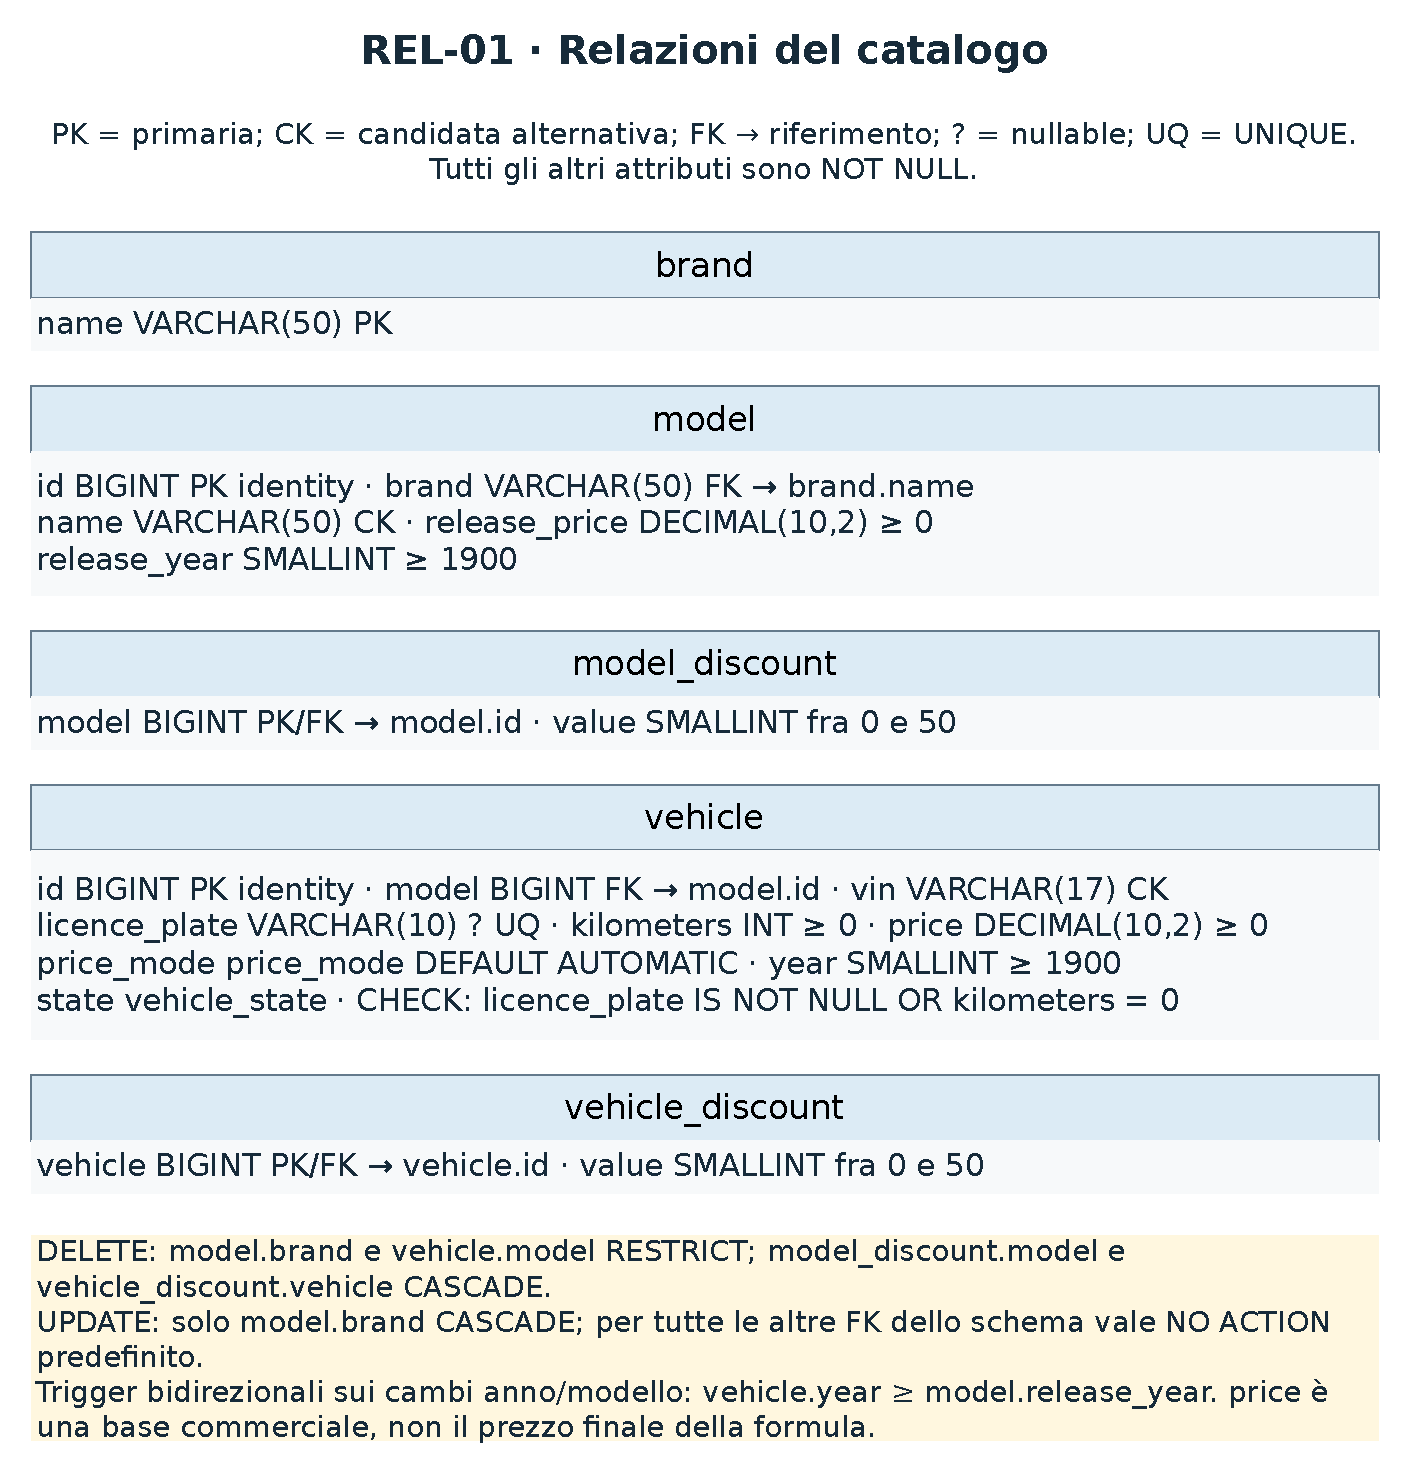
\includegraphics[width=\linewidth,height=.88\textheight,keepaspectratio]{diagrammi/database-relazionale-catalogo.drawio.pdf}
  \caption{REL-01 --- Attributi, chiavi e vincoli delle cinque tabelle del catalogo.}\label{fig:rel01}
\end{figure}
\begin{figure}[p]
  \centering
  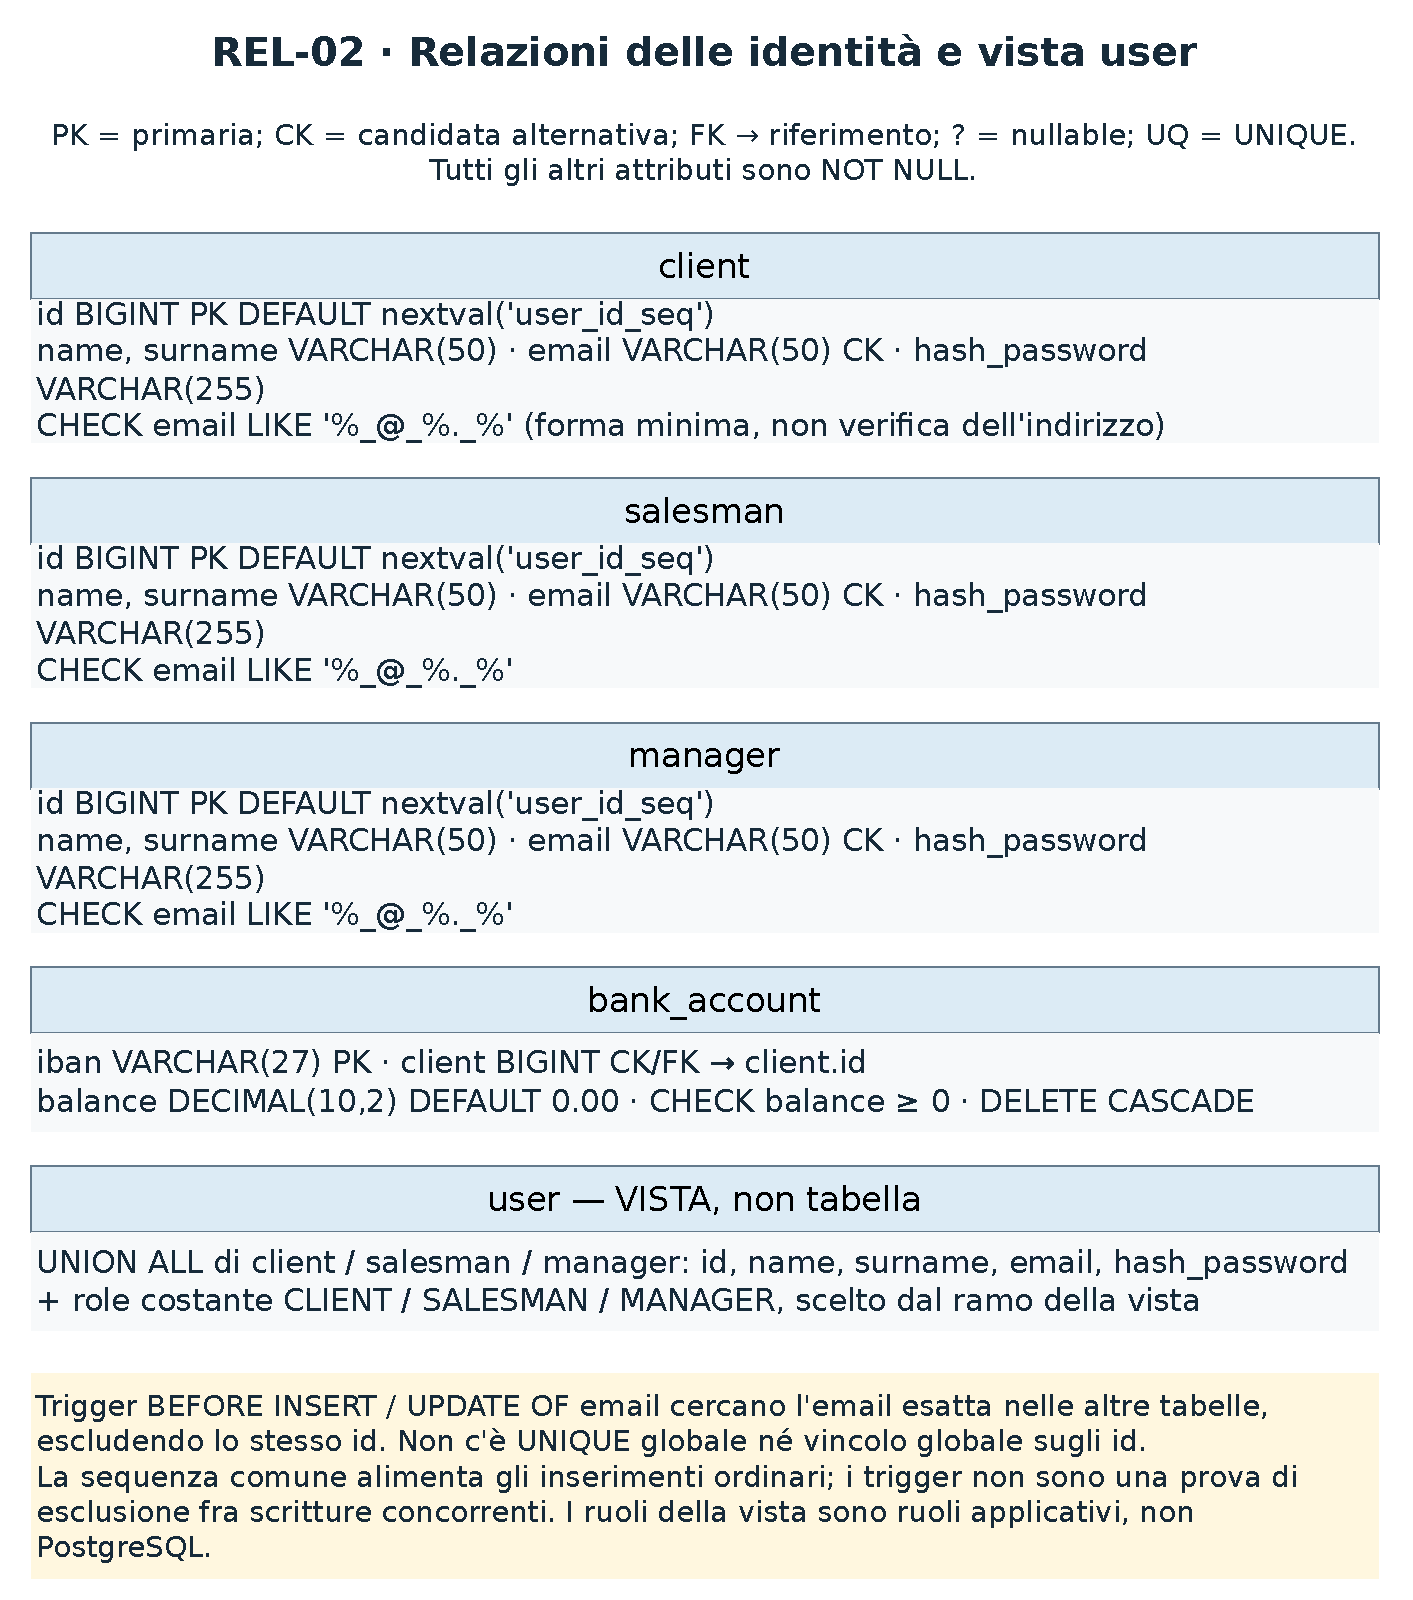
\includegraphics[width=\linewidth,height=.88\textheight,keepaspectratio]{diagrammi/database-relazionale-identita.drawio.pdf}
  \caption{REL-02 --- Tre tabelle di ruolo, conto dimostrativo e vista delle identità.}\label{fig:rel02}
\end{figure}
\begin{figure}[p]
  \centering
  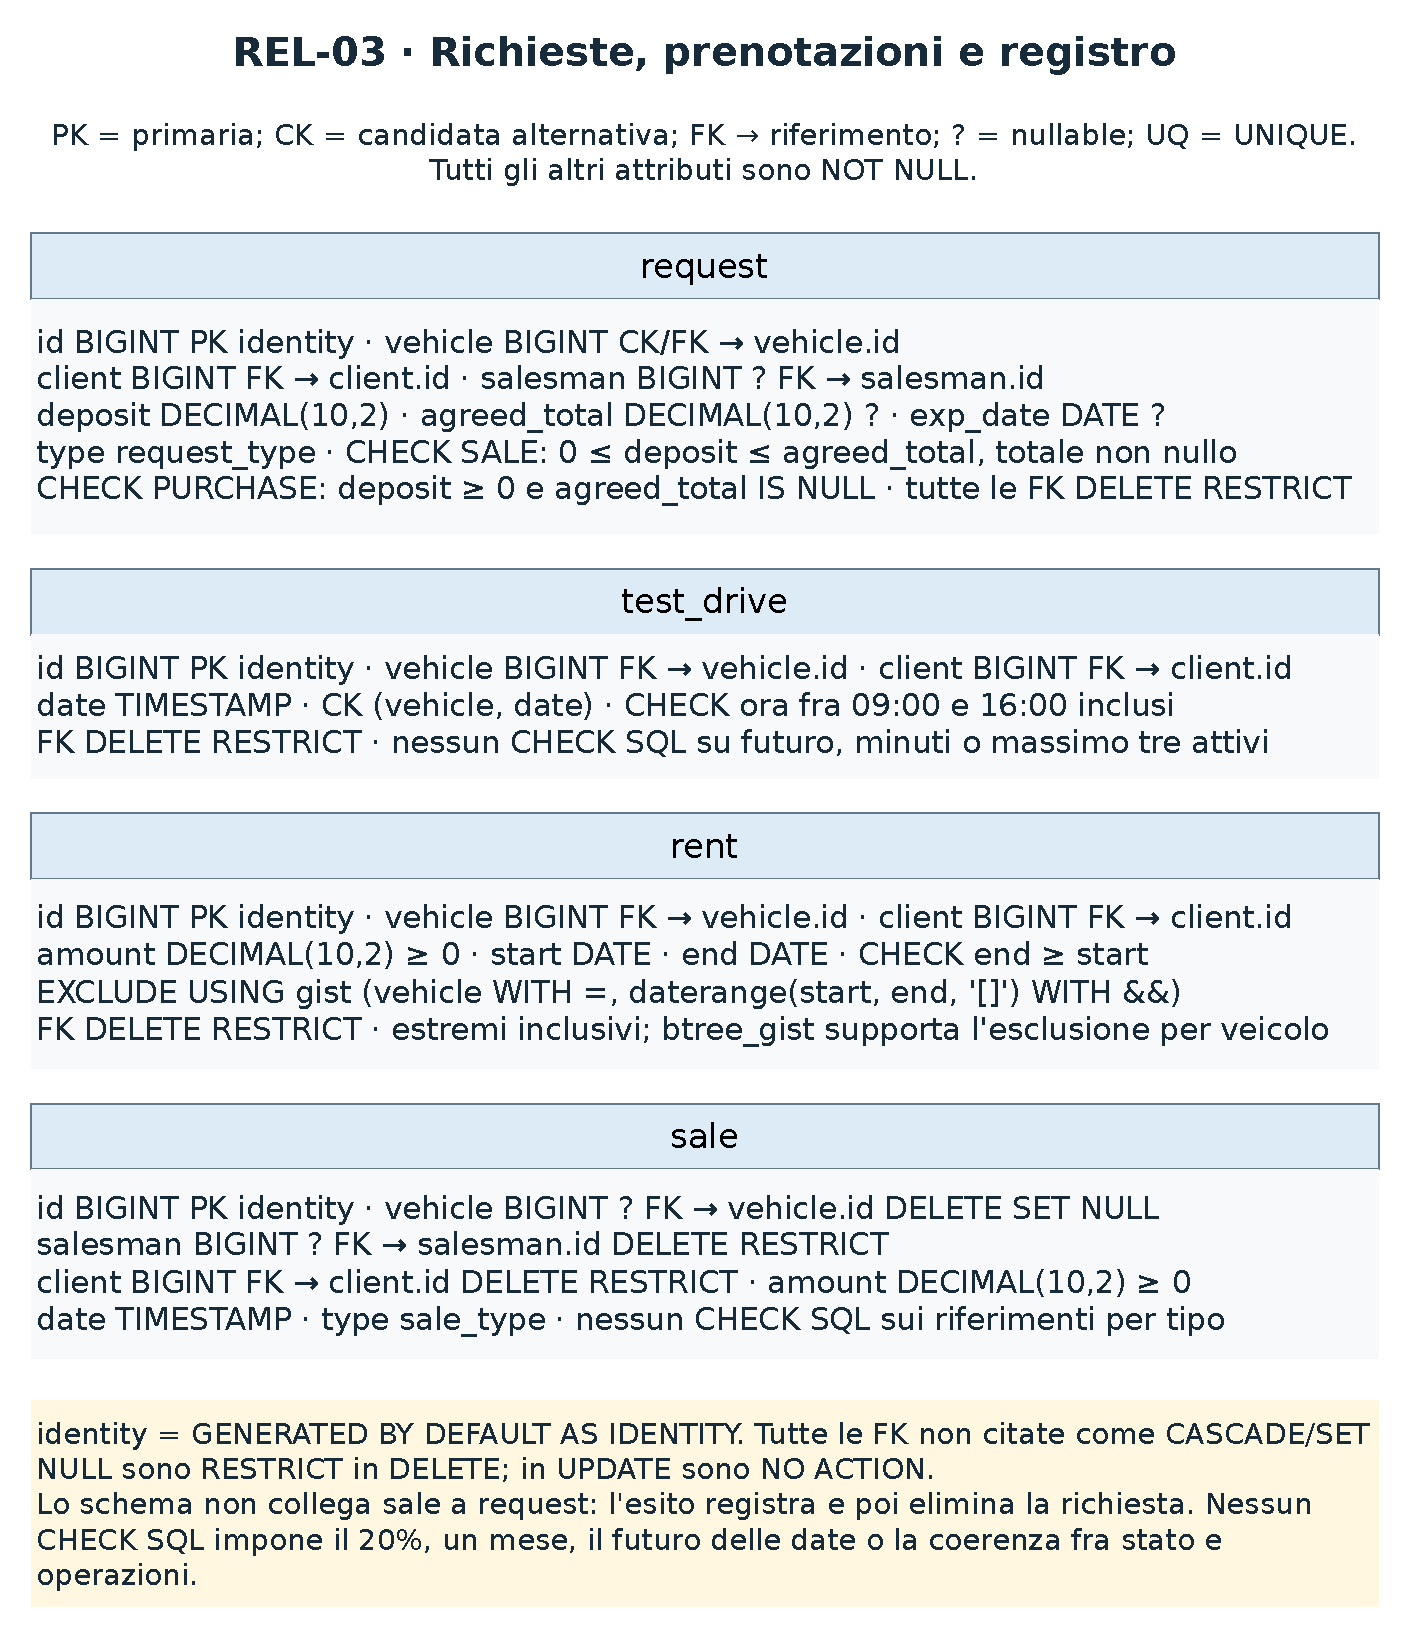
\includegraphics[width=\linewidth,height=.88\textheight,keepaspectratio]{diagrammi/database-relazionale-operazioni.drawio.pdf}
  \caption{REL-03 --- Richieste, test drive, noleggi e registro economico.}\label{fig:rel03}
\end{figure}
\clearpage

L'ADR~0002 mantiene quattro tipi enumerati nativi PostgreSQL, ciascuno
distinto. \code{vehicle\_state} ammette \code{SALE} (destinato alla
vendita al cliente), \code{RENT} (destinato al noleggio), \code{BLOCKED}
(riservato per la vendita al cliente), \code{WAITING} (proposta di cessione
in valutazione) e \code{SOLD} (venduto al cliente).
\code{request\_type} ammette \code{SALE} per la richiesta di vendita
al cliente e \code{PURCHASE} per quella di acquisto dal cliente.
\code{price\_mode} distingue \code{AUTOMATIC}, con base del modello,
da \code{MANUAL}, con base del veicolo nella stessa formula.
\code{sale\_type} distingue \code{SALE}, \code{PURCHASE} e
\code{PENALTY}: vendita al cliente, acquisto dal cliente e penale.
Il tipo esplicito determina il significato economico, anche a importo zero.
Non sono ruoli né stati di una richiesta. I DAO effettuano i cast JDBC
verso gli enum SQL e ricostruiscono gli enum Java; la scelta non richiede
qui nuove conversioni o migrazioni.

Gli importi persistenti usano \code{DECIMAL(10,2)}. I \code{CHECK}
impongono prezzi di rilascio e basi del veicolo, saldo, importo del
noleggio e importo del registro non negativi. Per \code{request},
\code{ck\_request\_agreement} distingue due forme: \code{SALE} richiede
totale non nullo, acconto non negativo e non superiore al totale;
\code{PURCHASE} richiede stima non negativa e totale nullo.
Il database non impone acconto del 20\%, immutabilità dell'accordo nel
tempo, associazione con lo stato del veicolo o corrispondenza fra scadenza
e venditore. Dominio e servizi fissano e utilizzano l'accordo come mostrato
in SQ-01a/SQ-01c. Il registro non ha una FK alla richiesta: conserva
l'esito economico mentre la richiesta viene eliminata.

Altri \code{CHECK} limitano sconti interi a 0--50, chilometri non
negativi, anni almeno 1900 e assenza di targa soltanto con chilometri zero.
I trigger sull'inserimento o modifica di anno/modello del veicolo e sulla
modifica dell'anno di rilascio del modello controllano
che l'anno del veicolo non preceda quello di rilascio del modello.
La presenza di questi controlli non prova un isolamento serializzabile
di ogni modifica concorrente fra tabelle.

Per la disponibilità, \code{rent} impone fine non precedente all'inizio
e un \texttt{EXCLUDE USING gist} sul veicolo e sull'intersezione di
\code{daterange(start,end,'[]')}, con estremi inclusi e supporto
\code{btree\_gist}. Due prenotazioni dello stesso veicolo non possono
condividere neppure un giorno. Il test drive rende unica la coppia
veicolo--timestamp e limita l'ora a 09:00--16:00 inclusi; non impone
slot interi di un'ora. Date future, limite di tre test drive attivi,
stato compatibile del veicolo e conflitto test drive--noleggio sono
controlli di dominio, servizi e query DAO, non vincoli SQL trasversali.
Le date del registro e dei test drive sono \code{TIMESTAMP} senza fuso;
quelle di noleggio e scadenza sono \code{DATE}. Il DDL non vieta date
nel passato né date future nel registro. Il mese per il saldo e
l'innesco della gestione delle scadenze restano applicativi.

\subsection{Utenti, vincoli e semplificazioni}
\guillemotleft{}Utenti\guillemotright{} indica le identità applicative, non account PostgreSQL.
\code{client}, \code{salesman} e \code{manager} ripetono gli attributi
comuni; la vista \code{user} ne combina le righe con \texttt{UNION ALL}
e aggiunge il ruolo costante del ramo. \code{PostgresUserDao} usa quel
ruolo per costruire il sottotipo Java e indirizzare le scritture.
La sequenza condivisa \code{user\_id\_seq} assegna normalmente ID
distinti, ma le PK sono locali e il DDL consente ID espliciti:
non esiste una primaria globale fra ruoli né una tabella padre che
imponga da sola una generalizzazione totale ed esclusiva.

Ogni tabella di ruolo ha email obbligatoria e unica e un controllo
minimo di forma con \code{LIKE}. I trigger cercano email uguali nelle
altre due tabelle durante inserimento e modifica dell'email, escludendo
righe con lo stesso ID. Sono controlli procedurali, non un indice unico
globale: non dimostrano esclusione di scritture concorrenti e non
impediscono il caso di ID espliciti coincidenti. Il confronto SQL dei
vincoli è testuale, mentre la ricerca di accesso usa \code{LOWER(email)};
non si presenta quindi l'intero sistema come un'unicità globale senza
distinzione di maiuscole. Questi limiti sono segnalati separatamente,
senza introdurre uno schema alternativo.

Le password sono rappresentate da hash, non da credenziali in chiaro
nel modello documentato. La registrazione ordinaria crea solo un cliente
e il relativo conto a saldo zero nella stessa transazione.
Il conto ha IBAN come chiave, un solo cliente e saldo non negativo;
è una simulazione locale, senza collegamento bancario, verifica di
titolarità reale o registro separato di tutti i movimenti. Il formato
dell'IBAN è controllato dal dominio, mentre il DDL ne limita lunghezza
e unicità. La cancellazione del cliente elimina il conto per
\code{CASCADE}, anche se positivo, ma richieste e operazioni storiche
possono impedirla con le loro FK. L'accesso JDBC usa la connessione
configurata per l'applicazione: il DDL non crea un ruolo PostgreSQL per
ogni cliente, venditore o manager e non definisce politiche per riga.

Le scelte privilegiano un archivio didattico compatto, mapping JDBC
esplicito e riferimenti storici conservati. Non costituiscono una
contabilità bancaria completa né una garanzia generale di autorizzazione
o concorrenza. Schema corrente e quattro enum restano quelli consegnati,
coerenti con gli ADR~0001 e~0002; nessuna migrazione o conversione è
introdotta dalla relazione. Il capitolo 2 è ora completo e proposto,
con le appendici A--B, per la revisione degli autori; tale revisione
non è già approvata.
